\documentclass[10pt, twocolumn]{article}\usepackage[]{graphicx}\usepackage[]{color}
%% maxwidth is the original width if it is less than linewidth
%% otherwise use linewidth (to make sure the graphics do not exceed the margin)
\makeatletter
\def\maxwidth{ %
  \ifdim\Gin@nat@width>\linewidth
    \linewidth
  \else
    \Gin@nat@width
  \fi
}
\makeatother

\usepackage{Sweavel}


\usepackage[breaklinks=true]{hyperref}
\usepackage{url}
\usepackage[a4paper, margin = 1.5cm]{geometry}
\usepackage{a4wide}
\usepackage{float}
\usepackage[english]{babel}
\usepackage[utf8]{inputenc}
\usepackage{amsmath}
\usepackage{amssymb}
\usepackage{xspace}
\usepackage[backend=bibtex,style=numeric-comp,sorting=none]{biblatex}
\usepackage{color}
\usepackage{csquotes}

\bibliography{spa3}
\usepackage{subcaption}
\usepackage[font={small}]{caption}
\usepackage{booktabs}
\usepackage{listings}
\usepackage{cleveref}
\usepackage{lipsum}
\newcommand{\approxtext}[1]{\ensuremath{\stackrel{\text{#1}}{=}}}
\newcommand{\matr}[1]{\mathbf{#1}}
\newcommand{\partt}[2]{\ensuremath{\dfrac{\partial {#1}}{\partial {#2}}}}
\renewcommand{\d}[1]{\ensuremath{\operatorname{d}\!{#1}}} % non-italized differentials
\newcommand{\h}[0]{\ensuremath{\hbar}} % hbar
\def\changemargin#1#2{\list{}{\rightmargin#2\leftmargin#1}\item[]}
\let\endchangemargin=\endlist 
\usepackage{amsthm}
\theoremstyle{plain}
\renewcommand{\theequation}{\thesection.\arabic{equation}}
\def\changemargin#1#2{\list{}{\rightmargin#2\leftmargin#1}\item[]}
\let\endchangemargin=\endlist    
\newcommand{\ts}{\textsuperscript} 
% Stephen's stuff
\newcommand{\R}{\texttt{R}}
\newcommand{\Rfunction}[1]{{\texttt{#1}}}
\newcommand{\Robject}[1]{{\texttt{#1}}}
\newcommand{\Rpackage}[1]{{\mbox{\normalfont\textsf{#1}}}}
\usepackage{xcolor}
\definecolor{Red}{rgb}{0.7,0,0}
\definecolor{Blue}{rgb}{0,0,0.8}
\hypersetup{%
pdfusetitle,
bookmarks = {true},
bookmarksnumbered = {true},
bookmarksopen = {true},
bookmarksopenlevel = 2,
unicode = {true},
breaklinks = {false},
hyperindex = {true},
colorlinks = {true},
linktocpage = {true},
plainpages = {false},
linkcolor = {Blue},
citecolor = {Blue},
urlcolor = {Red},
pdfstartview = {Fit},
pdfpagemode = {UseOutlines},
pdfview = {XYZ null null null}
}
%% Listings
\lstset{ 
language=R,                     % the language of the code
basicstyle=\footnotesize,       % the size of the fonts that are used for the code
numbers=left,                   % where to put the line-numbers
numberstyle=\tiny\color{gray},  % the style that is used for the line-numbers
stepnumber=1,                   % the step between two line-numbers. If it's 1, each line will be numbered
numbersep=5pt,                  % how far the line-numbers are from the code
backgroundcolor=\color{white},  % choose the background color. You must add \usepackage{color}
showspaces=false,               % show spaces adding particular underscores
showstringspaces=false,         % underline spaces within strings
showtabs=false,                 % show tabs within strings adding particular underscores
rulecolor=\color{black},        % if not set, the frame-color may be changed on line-breaks within not-black text (e.g. commens (green here))
tabsize=2,                      % sets default tabsize to 2 spaces
captionpos=b,                   % sets the caption-position to bottom
breaklines=true,                % sets automatic line breaking
breakatwhitespace=false,        % sets if automatic breaks should only happen at whitespace
title=\lstname,                 % show the filename of files included with \lstinputlisting;
% also try caption instead of title
keywordstyle=\color{Blue},      % keyword style
commentstyle=\color{orange},    % comment style
stringstyle=\color{Red},        % string literal style
escapeinside={\%*}{*)},         % if you want to add a comment within your code
morekeywords={*,...}            % if you want to add more keywords to the set
} 
\usepackage{verbatim}
\usepackage{multicol}
\def\changemargin#1#2{\list{}{\rightmargin#2\leftmargin#1}\item[]}
\let\endchangemargin=\endlist
\addtolength{\oddsidemargin}{-.35in}
\addtolength{\evensidemargin}{-.35in}
\addtolength{\textwidth}{.7in}

%%%%%%%%%%%%%%%%%%%% Begin
\title
{
%\phantom{a}\vspace{2cm}
\textbf
{
Scientific Programming: Assignment 3}\\[1em]
\small{University of Cambridge}
}

\author{Henrik Åhl}
\date{\today}
\renewcommand{\textfraction}{0.05}
\renewcommand{\topfraction}{0.8}
\renewcommand{\bottomfraction}{0.8}
\renewcommand{\floatpagefraction}{0.75}
\makeatletter
\makeatother
\makeatletter
\def\blx@maxline{77}
\makeatother

\newcommand{\ga}{genetic algorithm\xspace}
\newcommand{\sa}{simulated annealing\xspace}
\newcommand{\kh}{SOFM\xspace}

\begin{document}

% # <<libraries, echo = FALSE, message = FALSE, warning = FALSE>>=
% #   # Input libraries
% # @
% \date{\today}
\maketitle
% \setcounter{page}{1}
% \begin{abstract}
% {\bf -- yeah!
% }
% \end{abstract}
\section*{Preface}
This is an assignment report in connection to the \textit{Scientific Programming} module in the Computational Biology MPhil progeamme at the University of Cambridge, Michaelmas term 2016. All related code is as of \date{\today} available per request by contacting the author at \href{mailto:hpa22@cam.ac.uk}{hpa22@cam.ac.uk}.

\section{The Travelling Salesman Problem}
The Travelling Salesman Problem (TSP) is an NP-hard problem where a fictionary salesman wishes to travel past every city in a network such that every city is visited exactly once, and then return from the city of origin. The salesman also wishes to do this the fastest way possible, and thus seeks to find the shortest path such that the conditions are fulfilled. 
  
In our version of the TSP, we utilise the problems found at the Ruprecht-Karls-Universität Heidelberg TSPLIB database~\cite{tsplib}, and choose to seek an optimal path in all the two-dimensional euclidian problems with known, mathematically proven optimal solutions. Our individuals are defined as \R \textit{list} objects, containing a tour and its corresponding fitness (cost). 

We measure fitness in all of our implementations by considering the \textit{cost} of a solution -- in our case the total euclidian distance between the nodes in our given networks. As our implementations by design are not dependent on the cost aside from a greater than--lower than perspective, we do not normalise our measure (see below). The general encoding is defined as a vector containing integers corresponding to node indices, i.e.\ one index per node. All parameters were chosen through manual optimisation, i.e.\ a testing-correcting procedure.

%% Genetic algorithms
  \subsection{Genetic Algorithm Design}
    \paragraph{Mutation operator}
      We consider multiple mutation operators in this assignment. Key is that we initially mainly are interested in producing solutions widely different from our own, and later on solutions that swap or move longer connected circuits. We consider three separate operators, partly inspired by approaches mentioned by Larra{\~{n}}aga et al.~\cite{ga_tsp} as well as by Schneider~\cite{sa_tsp}: 
      \begin{description}
        \item{\bf Chunk mutation} Two integers in the range of the tour length are drawn randomly. The bases in between of these indices are selected and moved to an interval determined by a new random number, which signifies the start position of the chunk.
        \item{\bf Swap mutation} For every base in the sequence a random number is drawn. If this number is lower than a defined \textit{mutation probability}, the number is added to a pool. All the numbers into this pool are then shuffled and reinserted. For our mutation probability, we use the rate $1 / 2C$, where $C$ is the number of cities in the map.
        \item{\bf Reverse mutation} Two indices are again drawn randomly. The sequence is then inverted and inserted, e.g.\ the subsequence (red) 3-{\color{Red}5-2-4}-1 being selected would return the sequence 3-{\color{Red}4-2-5}-1.  
      \end{description}
      
      Testing various approaches shows that using several different operators is too computationally intensive for making the approach comparable to \sa. We therefore in our latter analyses restrict ourselves to using only our \textit{reverse mutation} operator. The settings then used consist of a population size of 14, where 90~\% (12) of these undergo mutations every iteration. Similarly, 20~\% (2) undergo crossover. Which individuals are selected for these operations is like the survival based on a tournament selection procedure (see below).
      
    \paragraph{Crossover operator}
      For our crossover operator we are interested in finding a way to preserve loops, but otherwise retain the current structure. We therefore implement our version of what we denote as \textit{pillar crossover}. In this process, we take two individuals, draw two random indices where the bases in between are kept. The lacking bases are taken from the other individual in the sequence they are found such that no already included bases will appear. For the other offspring, the inverse is applied, where all the bases aside from those in the prior region are kept, and bases from the first offspring then inserted into the gap. This process is inspired by Jacobson~\cite{crossover}.
      
    \paragraph{Selection operator}
      We apply coupled elitistic ($n = 1$) and pairwise tournament selection, i.e.\ for every generation, we keep the most fit individual, and draw from the remaining subset iteratively two random individuals where we then choose the subject for survival from a binomial distribution ($p=1$) until a full population is produced. That is, we always keep the best solution of the whole population, as well as the best individuals in the pairs.
      
%% Simulated annealing
  \subsection{Simulated Annealing Design}
    \paragraph{State alteration}
      New states are produced through the same procedure as in the \ga \textit{reverse mutation}, though also the . 
      \textit{chunk mutation} operator is tested; simulations do however give better results with the prior approach. 
    \paragraph{Temperature}
      Initial temperature is set to 1000$^\circ$~Å\footnote{Degrees Åhl}. Temperature is decreased exponentially, with a rate factor of $k = 0.9999$ per iteration. 

  \subsection{Comparison}
  We simulate both of our algorithms on euclidian two-dimensional tours for 30 minutes, as both methods have in general converged at that point. Both approaches do a fairly good job with finding good solutions to the problem. However, none of the algorithms are particularly good at finding the global optimum, even though they typically get fairly close. Simulated annealing tends to have a much faster convergence towards a near-optimal state with respect to runtime, whereas the genetic algorithm converges more slowly, due to the higher computational effort needed. 
  
\Cref{fig:comp} shows the end results for the algorithms after 30 minutes runtime,  As the result suggest, both methods produce very similar results in most cases, aside from the one tour with contains a very large number of nodes. Nevertheless, simulated annealing consistently performs slighlty better than the genetic algorithm, although it is likely that these differences mainly lie with respect to the design choices made, and not the intrinsic nature of the algorithms themselves; a 1-sized genetic algorithm with fitness-based selection should be comparable to simulated annealing. Also, reducing the selective pressure for the genetic algorithm should introduce more diversity, and possibly better results. However, this introduces another variable to configure, and would likely require a significantly larger population size, which would decrease the optimisation speed. 
  
\begin{Schunk}
\begin{figure}[H]

{\centering 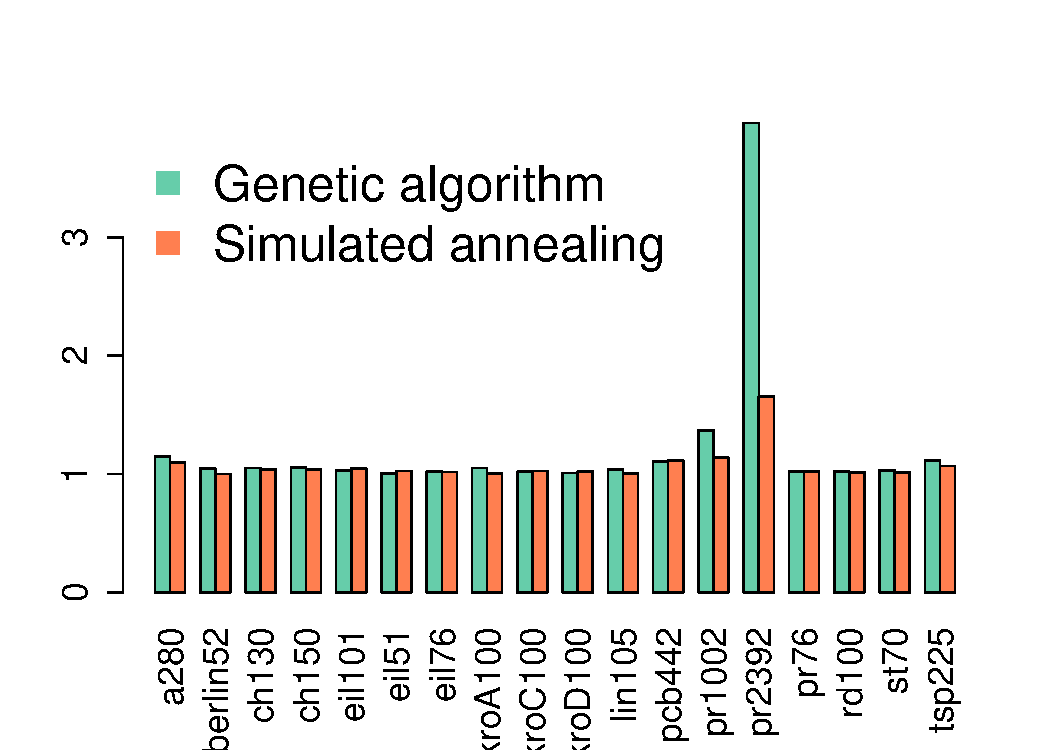
\includegraphics[width=\maxwidth]{figure/twocolumn-comp-1} 

}

\caption[Performance comparison between genetic algorithms and simulated annealing, having run the simulations for 30 minutes]{Performance comparison between genetic algorithms and simulated annealing, having run the simulations for 30 minutes. The fraction shown is the fractional distance travelled as opposed to the optimal tour. Only one simulation manages to completely solve the problem, namely the simulated annealing method in the \textit{berlin52} setting.}\label{fig:comp}
\end{figure}
\end{Schunk}

We should also note that while the scaling of error measure used here does not affect the \ga design in any direct way, as our selection is deterministic in the comparative step. However, as soon as a probabilistic approach is introduced, we would have to account for this. In the case of simulated annealing the error measure already affects the parameter setup, i.e.\ the temperature and the cooling schedule.  


\section{The Kohonen Self-Organising Feature Map}
  \subsection{Weight Distribution in Output Space}
    The Kohonen \kh is designed utlising a rectuangular grid and linear learning factor decay. Being aware of the benefits in choosing an appropriate initial distribution of our weight nodes, we disregard this in favor of mimicking the setup used by Beale and Jackson~\cite{neuralnets}, i.e.\ a random initial distribution centered within weight-space. In this initial exercise, we generate one data point per iteration, and modify our network accordingly.
    
    As can be seen in figure~\cref{fig:shapes}, the ability of the grid to arrange itself according to the input space is heavily dependent on the parameters used. In the first row, the \kh is able to neatly align itself according to its uniform two-dimensional input, whereas in the other cases, we are less successful. As all input is already on the same scale and of the same type, we do not bother with vector normalisation.
    
    We can infer from our selection of simulations that the initial distribution is undoubtedly important. In particular, we can see how the neighbourhood is plays a significant role in breaking the initial distribution of nodes. When this does not happen, nodes can get trapped with the wrong setup relative to each other, as is particularly evident in \cref{fig:shapes} rows 2 and 4. In contrast, row 3 shows a distribution tending towards the correct one, but is unable to break loose of the clusters due to the size of the neighbourhood. In principle they ultimately will as long as their relative position is correct with respect to the input distribution, but the time required for this depends largely on the learning rate.
    
    \begin{figure*}[p]
      \centering
      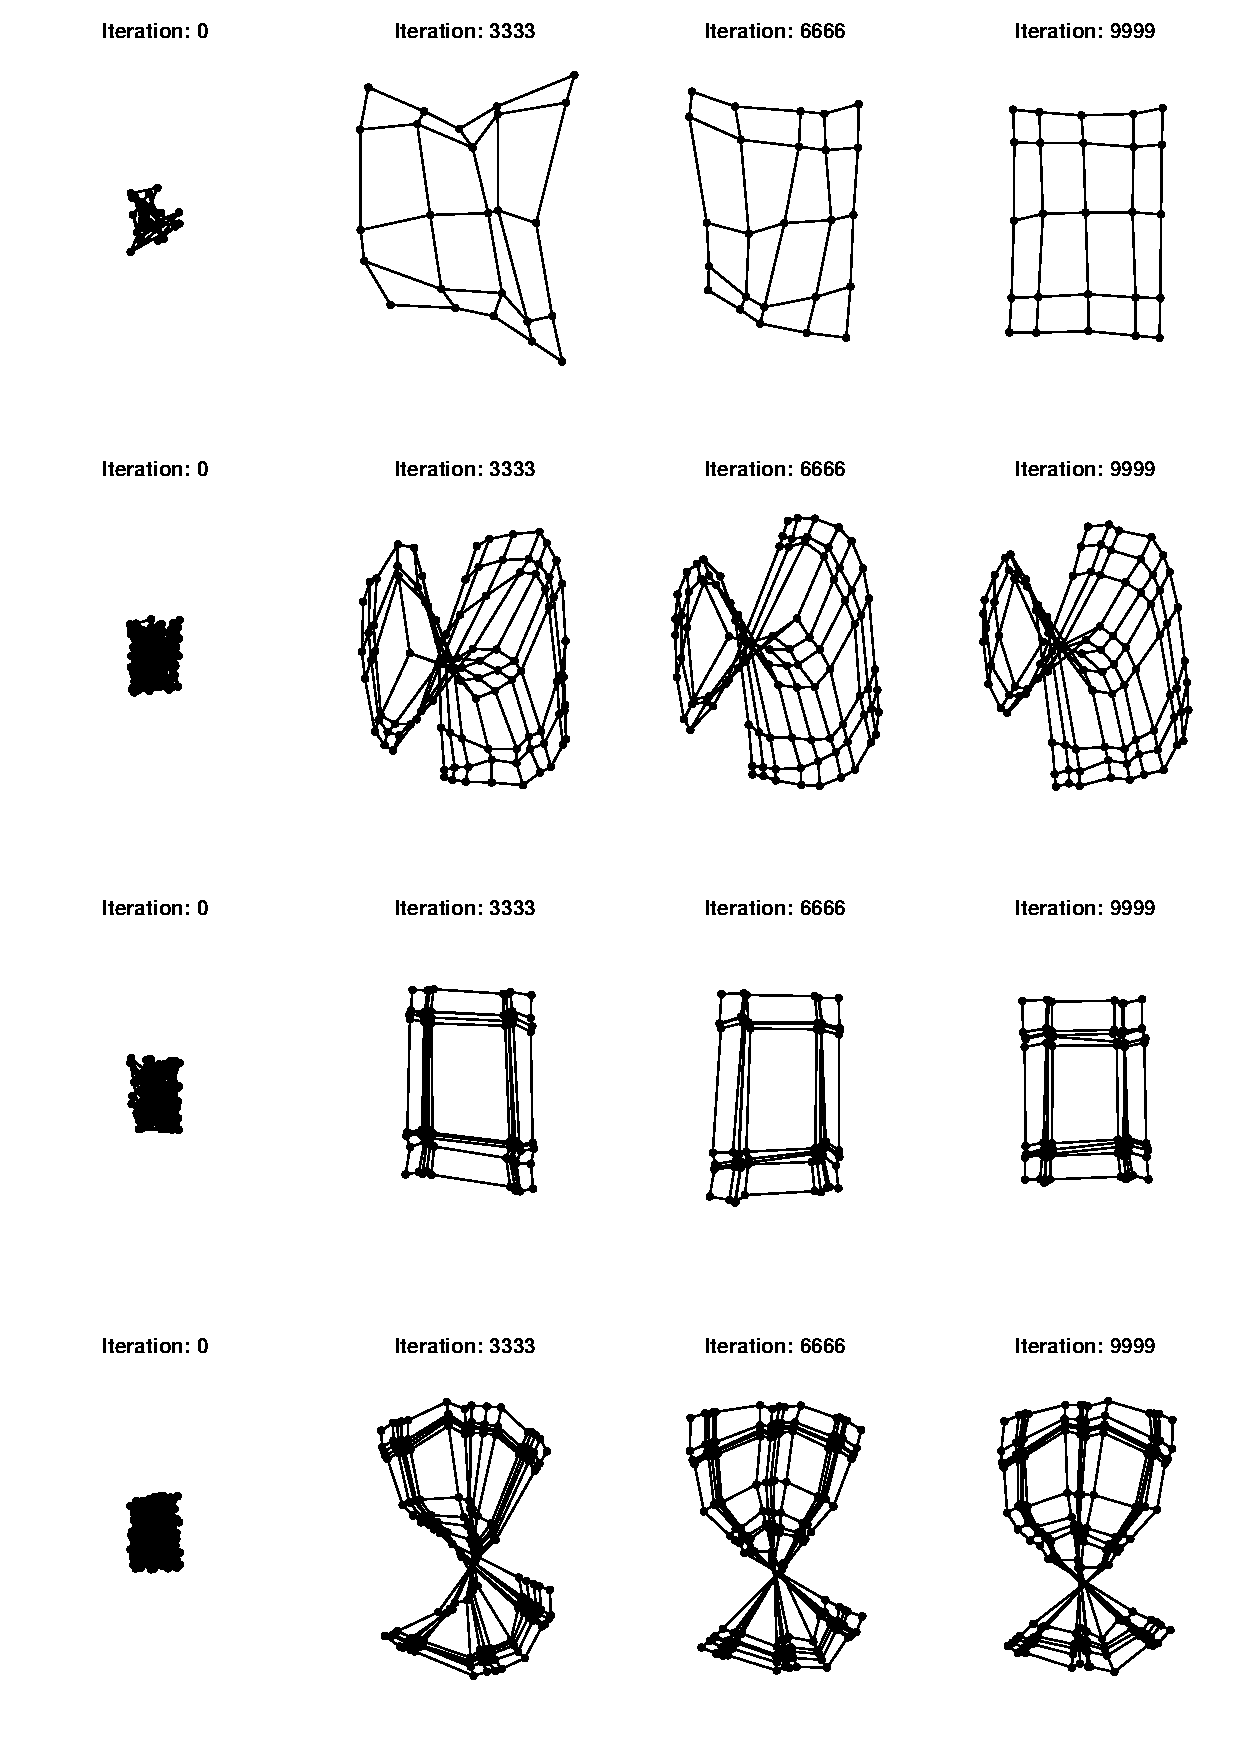
\includegraphics[scale=.7]{koh_shapes.pdf}
      \caption{Shapes in weight-space produced by the Kohonen SOFM. The rows show various configurations of parameters, namely $\{0.5, 0.05, 0.03, 0.01\}$ for the learning rate (with a final rate of 0.01),  $\{25, 100, 100, 225\}$ for the number of nodes (square grid), and $\{2, 3, 5, 5\}$ for the initial neighbourhood, in order. In all figures, the input consists of uniform, randomly generated 2D data.}
      \label{fig:shapes}
    \end{figure*}
    
  \subsection{SOFMs for Image Compression}
    \subsubsection{SOFM Design and Test Images}
    For image compression, we apply our approach to two separate images: the common \textit{Lena} image, featuring Swedish playmate Lena Söderberg, as well as an image of Italian actor and fashion model Fabio Lanzoni. These both consist, after modification, of $512 \times 512$ pixel lossless images (.tiff and .webp respectively), which are translated into their RGB colour channels in \R using the \texttt{pixmap} and \texttt{webp} packages.
  
  The images are encoded in the \kh using either $4 \times 4$ or $8 \times 8$ bases large flattened input vectors, corresponding to same-sized pixel blocks in the original images. For training of the network, we employ two strategies: 
  \begin{description}
    \item{\bf Uniform input} All input is looped over, passed into the \kh one block at a time, giving an overall equal representation of all the blocks in the image. 
    \item{\bf Random input} Random blocks in the original image is passed as input. 
  \end{description}
  
  In theory, it ought to be reasonable to consider a third approach, where the images vectors passed as input are done so corresponding to how prevalent they are in the original image, i.e.\ a frequently occurring block would need to be passed as input less often. However, due to the need to computationally assess the similarity between different blocks, we do not consider this approach practically, although it is likely that it would produce better results due to being able to account for details to a greater degree. 
  
  Also, as opposed to Amerijckx et al.~\cite{koh_img_comp}, who also used a DCT filter and a differential coding scheme, we have in our method only applied the \kh directly. Introducing those extra treatments are likely to further enhance the quality of the compression. It is also likely that the SOFM could be improved upond through the implementation of a neighborhood function which would allow for proportional adjustment of the nodes given their respective distance to the winning one in the selection step, as it possibly would prevent the occurence of nodes being locked "out of place", as we have seen can happen in~\cref{fig:shapes}. 

    \subsubsection{Comparison to Single-Value Decomposition}
      In order to compare our method to SVD, we utilise the implementation done by Myles~\cite{svd}. As we can see visually in~\cref{fig:comp}, both methods do a comparable job in compression when using a 30-worth SVD and a $4 \times 4$ block SOFM with 100 nodes. Still, it should be noted that the use of so many nodes was somewhat superfluous; similar results for the Lena image were attained using a mere 25 nodes. 
  
The quality of the compression is notably degraded when using random inputs, which seems to reinforce the bias towards the more prevalent blocks, or at least establishes further noise with respect to the ability to pick up details in more rarer chunks. Compared to SVD, the SOFM produces grainier images related to the overall amount of detail in the image, i.e. a blockwise graininess. The SVD method on the other hand produces graininess with respect to visual features, such as in the transition between the curtain and the arm in the Fabio image, which are both of similar hue. Having the ability of self-organisation, the Kohonen approach is in that sense more capable of accounting for point-wise details by clustering more nodes in the region of the image weight-space which is more variable.

As we can note in \cref{fig:koh_svd}, the Kohonen net and the SVD approach are somewhat different in their outcome with respect to file size. Even though the results have here been ported through PNG compression, we can see traits of the respective encodings. In the SVD case, we achieve a linear or logarithmic trend for file size with increasing decomposition values, whereas the Kohonen net is significantly more static. We can also see the probabilistic nature of the SOFM, alternating in file size independently of the number of nodes (and also without loss of visual quality; image not shown). Furthermore, while it can be said that the SVD compression is affiliated with higher visual quality of the images the higher the decomposition value, the same cannot the said of the SOFM. However, when using larger blocks sizes, e.g.\ $8 \times 8$ chunks, the quality quickly deteriorates. 

\begin{Schunk}
\begin{figure}[H]

{\centering 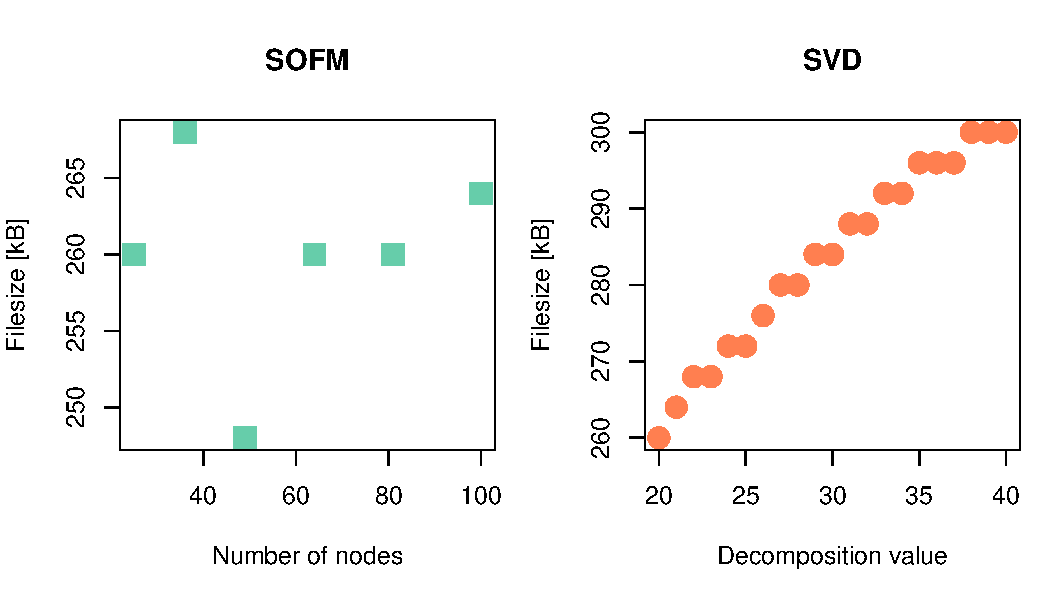
\includegraphics[width=\maxwidth]{figure/twocolumn-koh_svd-1} 

}

\caption[File sizes for images ported through PNG compression after their respective treatments]{File sizes for images ported through PNG compression after their respective treatments. Note the differing scales.}\label{fig:koh_svd}
\end{figure}
\end{Schunk}

Finally, we can consider the amount of information needed to store our data in~\cref{fig:comp}, where the visual quality is overall fairly comparable. In the Kohonen case we require $no.~nodes \times block~size + no.\ blocks = 17984$ pieces of information, whereas we for the SVD require $DV \times image~width + DV^2 + DV \times image~height = 31620$ pieces, compared to the 262144 pixels in the uncompressed image.

\printbibliography
 
    \begin{figure*}[t]
      \centering
      \includegraphics[scale=.6]{channels.pdf}
      \caption{Colour channels for the Lena and Fabio images. Lena is affiliated with more light and details, whereas Fabio has both a smoother background and more uniform lines in large.}
      \label{fig:channels}
    \end{figure*}~\begin{figure*}[b]
      \centering
      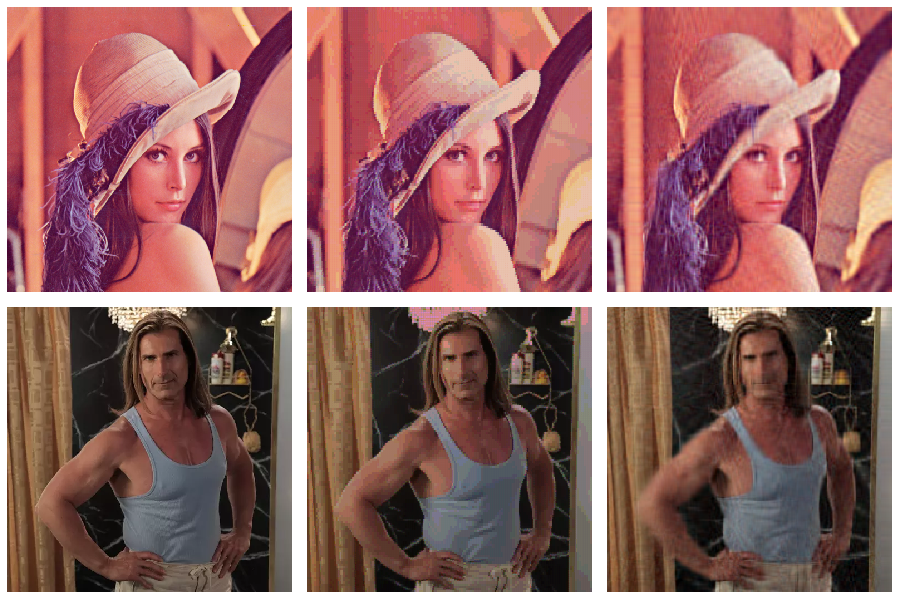
\includegraphics[scale=.6]{comp.pdf}
      \caption{Compression comparison for the different methods. The first column shows the uncompressed variants, whereas the second and third show compression using a $4 \times 4$ block SOFM (100 nodes), and compression using a 30-type SVD.}
      \label{fig:comp}
    \end{figure*}

\newpage
\onecolumn
  \appendix
\section{Code}
\lstinputlisting{ga.R}
\lstinputlisting{simann.R}
\lstinputlisting{koh.R}
\lstinputlisting{comp.R}

\end{document}
